\documentclass[reprint,unsortedaddress,amsmath,amssymb,aps,prl,showkeys]{revtex4-2}
\usepackage{graphicx}% Include figure files
\usepackage{dcolumn}% Align table columns on decimal point
\usepackage{subfigure}
\usepackage{bookmark}
% \usepackage\textbf{{biblatex}}\textbf{}
\usepackage{float}
\usepackage{url}
\usepackage{bm}% bold math
\usepackage{hyperref}% add hypertext capabilities
\usepackage[mathlines]{lineno}% Enable numbering of text and display math

\begin{document}

\title{Vicissitudes of Cities Driven by Re-distributive Growth}
\author{Gezhi Xiu, Jianying Wang, Lei Dong}
\author{Yu Liu}
\email{liuyu@urban.pku.edu.cn}
\affiliation{Institute of Remote Sensing and Geographic Information Systems (IRSGIS), Peking University}
\date{\today}

\begin{abstract}
    We propose a spatial growth model to address how cities emerge, grow, and especially, compete, with limited resource and space. The approach emphasizes on the evolutionary trajectory of cities, simultaneously determined by local (e.g., topography) and regional (e.g., industrial status) conditions, which can be attributed to the competition for redistributive resources in a given space. To model this spatial competition mechanism, our out-of-equilibrium growth model is set with a fixed bound on global growth rates. We discuss two phases of urbanization predicted in our model: (a) free growth phase, and (b) resource constrained phase. Zipf's and Clark's laws in urban sciences are found in (a), indicating realistic urbanization process has not yet reached bottlenecks of resource; And when it reaches, (b) captures the inevitability of various urban diseases, such as urban shrinkage in developed cities and the spatial relocation of developments. Our approach sheds light on analyzing urbanization with early warnings of environmental capacity.
\end{abstract}
\maketitle
% \section{Introduction}

% 研究的是一个什么问题(spatial growth model),这个问题为什么重要?(可以从理论和实践两个角度说,但偏重于理论)% 现在的研究做了什么(现在这块写得太宽泛了,其实相关工作很多,也很具体),有哪些不足?这些不足产生的「可能的」原因是什么?
\textit{Introduction.} Spatial growth models are powerful tools to understand urban growth dynamics~\cite{PhysRevX.4.011008, Li2017Simple, makse1995modelling, rybski2013distance, nanda2017spatial}. Theoretically, such models fill the gap between macroscopic patterns, e.g. socio-economic scalars and material properties, and microscopic dynamics, e.g. individual level interaction patterns; Practically, they investigate how different growth factors contribute to city emergence, and how these dynamics lead to some well-observed scaling law~\cite{bettencourt2007growth,court2013origins,batty2008size,batty2019urbanscalinglaw}, fractality~\cite{batty1994fractal,batty2007cities}, and city size distributions (i.e., Zipf's law)~\cite{zipf1949human}, making quantitative predictions broadly through urban morphology and spatial structures for urban planers and policy makers~\cite{anas1998urban}. These existing works have built natural paths in deriving macroscopic dynamical state from microscopic growth rules. Most of these approaches are based on the assumptions of homogeneous growth in Euclidean geometry. However, recent discoveries of complex spatial phenomena associated with realistic urban systems are better described using fractal or discrete geometry\cite{makse1995modelling,louf2014congestion,PhysRevE.58.7054}, to better consist with growth dynamics in disordered contexts and media. In words, urban space has memory of active components over it. The memory of the potentials to grow are spatially heterogeneous, and adding up which limited by the regional capacity. Such consistent heterogenity increases the significance of competition essence among cities, over ranking, spaces, and the number of employees. 

In this Letter, we introduce a spatial growth model based on inconsistent space and memory-based growth dynamics to describe how cities emerge, grow, and compete over given space and resource. The spatial sprawl of cities and the advance of urbanization are realized by the sequential settlement of new citizens. Here, the location choice of new citizens follows those active population of the whole region, and thus gives the physical form of each city by the exclusive and continuous area containing offspring citizens of the same ancestor. We show that beyond the desolated growth of each city, competitions introduced by spatial specialization and resource limit result in the vicissitudes of cities and urban shrinkage. Our model combines two themes for many disciplines, including probability theory and ecology: The spatial preferential attachment mechanism~\cite{Li2017Simple}, and the existence of environmental capacity under competition~\cite{gude2020bacterial,liu2019an}. 

On the first point, the \textit{rich get richer} mechanism is well-observed in social systems, especially, human settlements appear to be clustered hence cities~\cite{marsili1998interacting}. Literature has discussed how urban features emerge from preferential attachment via interaction density~\cite{ccolak2016understanding,louf2014congestion,fujita1976spatial}, e.g., multiplicative or correlated percolation~\cite{makse1995modelling,PhysRevE.58.7054,rybski2013distance}, spatial networks~\cite{marsili1998interacting,court2013origins,Li2017Simple}, and utility maximizing~\cite{PhysRevE.90.042815,axtell2001emergent}. Spatially, such mechanism leads to population clustering near every urban centers. Here, we take the spatial aspect from the idea of diffusion-limited aggregation~\cite{makse1995modelling, rybski2013distance, kleinberg2000navigation}, i.e., in each cities, new comers would settle near those active citizens.

On the second point, cities are systems with environmental capacity, that excessive employees do not guarantee the proportional urban output, considering the tradeoff in infrastructures and congestion. In words, the marginal effect of urbanization leads to decreases in urban attractiveness~\cite{atkinson2012urban, girardin2009quantifying,gomez2018explaining,parris2003characterizing,batty2008size}. These are poorly reflected in the referred works, which are mostly base on certain equilibrium conditions on growth rates or optimization aims~\cite{zipf1949human}, and predict constantly accelerating urbanization process. However, cities are inter-competitive and out-of-equilibrium to be consistent under circumstances towards sustainability\cite{fujita1976spatial,louf2014congestion,ccolak2016understanding}. Thus we include rules for spatial exclusiveness, and bounded growth rate in our model. Existing work has investigated in non-spatial context that systematic capacity puts severe constraints on the patterns of evolution~\cite{PhysRevE.55.R3817}. Here, our restriction are set to intensify inter-city competitions for active population\cite{batty2017urban}. We later prove that our space-relevant model extends the previous non-spatial predictions for city size distributions. These settings also result in realistic urban phenomena like superior switch\cite{gabaix2004evolution}, and urban shrinkage\cite{haase2014conceptualizing}, that cannot be formulated by existing growth models.

% 我们是怎么来解决这个问题的,有哪些重要的贡献。
%These concerns call for a general approach to model the spatial sprawl of emerging cities and their population under sustainable rules, regarding the competitions for space and resource.
% In brief, we propose an out-of-equilibrium spatial preferential growth model with restrictions on the maximum systematic growth rate. Existing work has investigated restrictions, non-spatial context proved that environmental capacity puts severe constraints on the patterns of evolution~\cite{PhysRevE.55.R3817}, such as fluctuations in city rank-size distribution. Our restriction setting is space-relevant, and is proved later to effectively enhance the intensity of competitions, 
% \section{Results}
% \subsection{The Spatial Yule Model}
% 我们提出了一个模型,能干什么事儿,有什么好处。

\textit{Spatial Yule Model.} Our model tells how cities emerge, grow, and compete over space. Its dynamics are mainly determined through three quantitative and spatial rules: 1) \textit{Active citizen rule}. During urban growth process, we assume that only 'active' citizens attract new comers to a nearby place in their city, $k$ and $N_i$ are the number of cities and active citizens in the $i$th city, respectively. 2) \textit{Memory kernel rule}. We take $\sum_{i} N_i \le N^*$ ($N^* \gg 1$) as the satiation condition, i.e., when the total population exceeds $N^*$, a new comer would deactivate a random dweller who is previously active. This mechanism keeps only up to $N^*$ active citizens. Therefore we say these $N^*$ people add up to the memory kernel. 3) \emph{Spatial growth rule}. We assume the studied area is an $L\times L$ 2-dimensional continuous space ($L\gg 1$) with grid of cells, %(IN THE BEGINNING, YOU SAID IT'S A continuous space?),
i.e., the locations of citizens are continuous, but the boundaries of cities are discrete on cells. A new city is seeded randomly over the region as a Poisson point process~\cite{miles1970homogeneous}, and survives if its cell is not taken; Every new citizen settles at a constant distance $r\le 1$ and a random angle $\theta$ from its introducer. Once a cell $c$ has held a citizen from the $i$th city, any citizens from another city $j$ ($j\ne i$) cannot introduce new comers on cell $c$. Thus cities are identified through citizens' ancestral introducer and their geographical occupation of blocks.

Based on these rules, we can define the model with a set of two-phase master equations. Specifically, we assume that the probability of a population increase in city $i$ within the time interval $(t,t+dt)$ is $\beta_2N_idt$, where $\beta_2$ is the introduction rate of every active citizen; We also assume that new cities constantly emerge with a small rate $\beta_1kdt$, proportional to the number of cities, where $\beta_1$ is the rate of new city generation. A city's generation is confirmed only if its location is at an empty cell. The master equation can therefore be written as \begin{align}\frac{\partial}{\partial t}N_i(t) =  \delta_{N_i(t)}\cdot k\beta_1+ (1-\delta_{N_i(t)})\cdot N_i\beta_2, \end{align} for the free growth phase, where urbanization is weakly dependent with space and resource $N^*$;
%[WHAT'S THE DEFINITION OF FREE GROWTH?], 
and \begin{align}
dN_i(t)/dt = \beta_2 N_i(t) -\delta_{\{\sum N_i = N^*\}}\cdot\notag \\ \left(\beta_1k(t) + (N^*-N_i(t))\beta_2 \right)
\end{align}
for the resource constraint phase, where the total resource $N^*$ are partitioned, and new dwellers get resource only through redistribution. 
%[WHAT'S THE DEFINITION OF RESOURCE CONSTRAINT PHASE?]. 

\begin{figure}
	\centering
	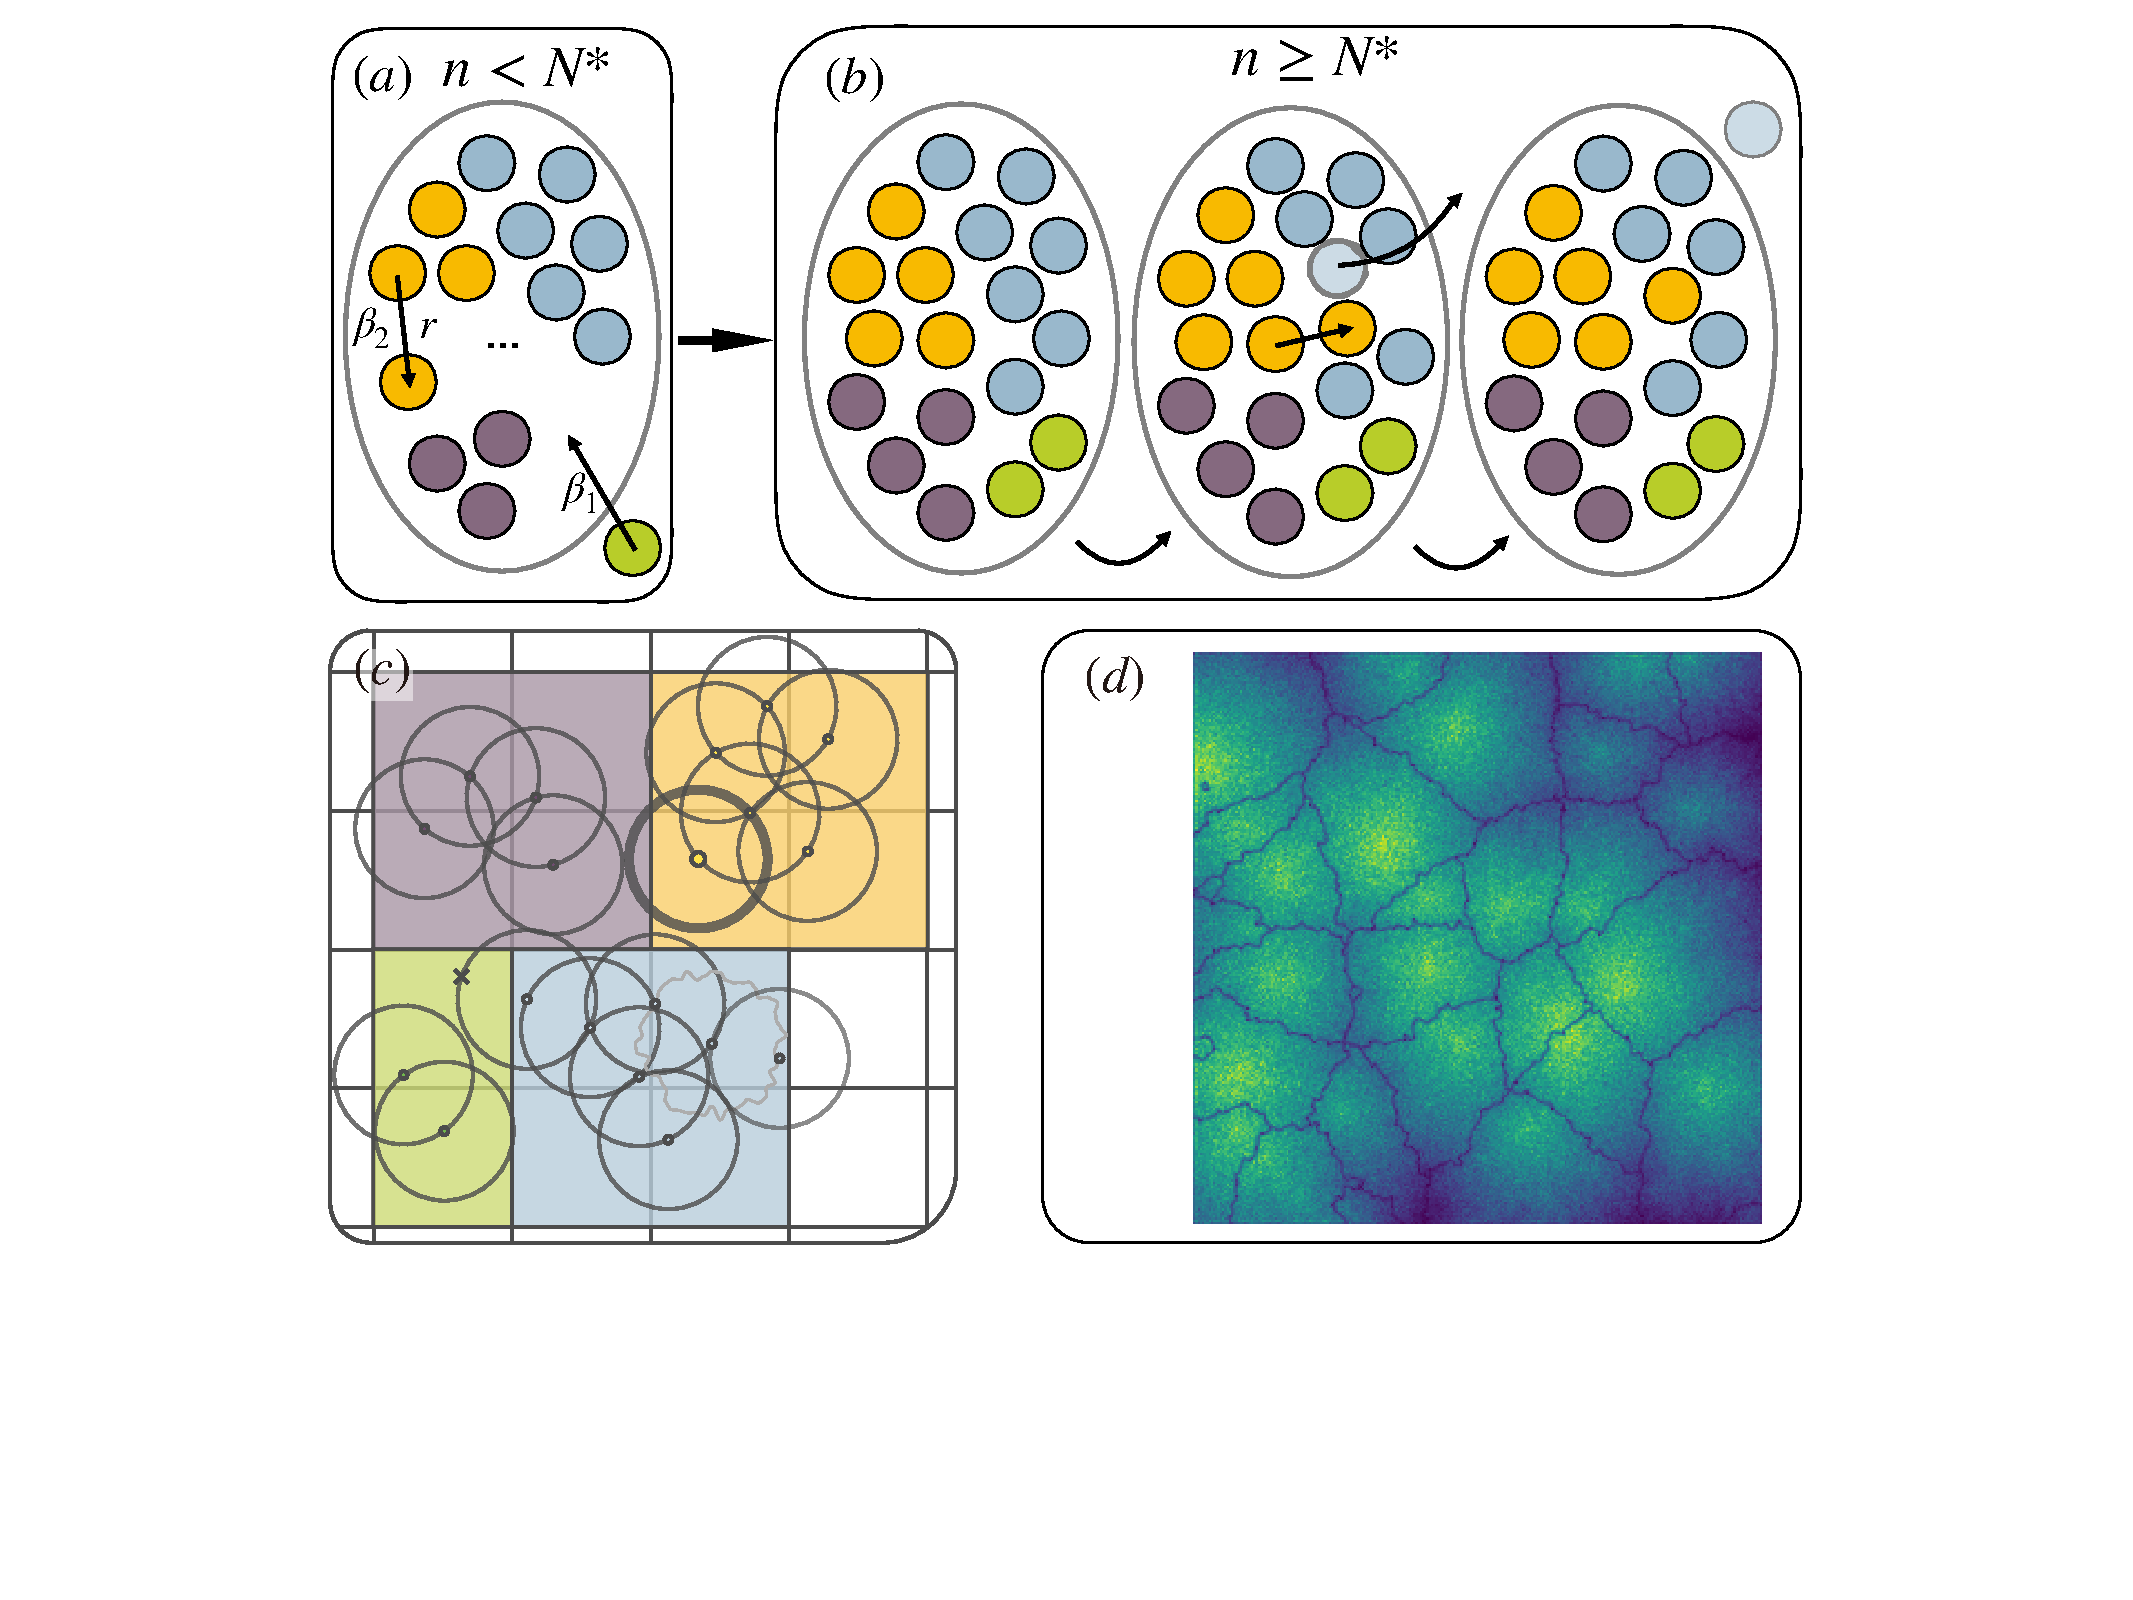
\includegraphics[width = 0.95\linewidth]{pics/sketchgood.pdf}
	\caption{\textbf{(a)} Status in the memory kernel at the free growth phase, i.e., the total population is less than $N^*$. Existing citizens introduce new dwellers at the rate $\beta_2$, while each existing city (noted by nodes in different colors) introduces new cities at the rate $\beta_1$. \textbf{(b)} When the memory kernel is fulfilled, every introduction of new city or citizen leads to an ejection of existing active citizen currently included in the memory kernel. \textbf{(c)} The spatial aspect is that, an offspring citizen's placement is at distance $r$ from the ancestral dweller. Also, when the kernel is filled, a new yellow node ejects an existed blue node, or equivalently deprive her ability to introduce. \textbf{(d)} A simulated result for $L$, $r$, $\beta$ equals to $256$, $0.5$, and $4$, respectively. We choose $\beta = 4$ to avoid confusion of too many cities. This is parallel to a quarter of $2L\times 2L$ simulation with $\beta = 1$.}
	\label{sketchpic}
\end{figure}

Though $\beta_1$, $\beta_2$ have their actual meaning of generation speed, the model's dynamics and patterns are only determined by the relative growth rate $\beta:= \beta_2/\beta_1$. This is parallel Yule's settings on modelling the distribution of species per genus~\cite{yule1925ii}.
%[WHY SET BETA? WHAT'S THE MEANING OF BETA], 
So our model could be regarded as a spatial Yule model with constraints (SYM). A sketch for the SYM is shown in Fig. \ref{sketchpic}.

% 5. 模型需要哪些假设 6. 这些假设有什么理论和实证基础?
% [THE FOLLOWING PARA IS VERY CONFUSING. IF THIS IS ALSO RULES, YOU SHOULD PLACE THEM IN THE ABOVE PARA. IF THIS IS NOT, YOU SHOULD SPLIT THEM AND INSERT INTO THE PLACE THAT INTRODUCE PARAMETERS.] 
The model implies some simple assumptions. First, urban developments are density-driven. Literature has suggested that density-driven social ties and interactions comprise an important driver of the economies of scale~\cite{pan2013urban, girardin2009quantifying, batty1992form}. In the SYM, we further assume only the density of attractive population is corresponding to urban developments. Such active part can be recognized as the total employed or productive people. Second, to make an analytic framework, the growth dynamics are set to be homogeneous. The choices of place of new comers are random; The rate of introduction and emergence is the same for every active citizen and every city. This diffusive setting of sequential settlements is also realistic urban growth~\cite{RevModPhys.87.925}. 

In the numerical experiments, which is elaborated in \textit{SI}, the truly worth-tuning parameters are three, $\beta$, $r$, and $N^*$. $\beta$ contributes to the Zipf's coefficient and later defined turnover rate~\cite{rooney2006structural}; $r$ contributes to the fractality of urban areas and the time to fill the whole space; $N^*$ is the severeness of resource competition. 
% 7. 这个模型能推出哪些结论(1,2,3)。这些结论能如何被数据验证。
% \subsection{The free growth phase}

\textit{The free growth phase.} SYM predicts the existence of three phases of regional growth of cities, distinguished by whether resource and space have been fully occupied: freely growth phase, economic constraint phase, and spatial constraint phase. We focus on the first two phases, which correspond with regional resource. Spatial constraint phase's evolution implies a fully urbanized area, which is unlikely seen in reality, we discuss the situation only in \textit{SI}. In the freely growth phase, cities grow desolately, without being limited by resource and space. In this phase, SYM reformulates two important properties, stately (1) Zipf's law~\cite{gabaix1999zipf's} for rank size distribution of cities' population, and (2) Clark's law for exponential decay of urban density\cite{clark1951urban}. 

The populations of cities typically decay proportionally to the inverse of their ranks~\cite{gabaix1999zipf's}. This is referred as Zipf's law of cities' population sizes, i.e., the populations of cities distribute as a power of ranks, $f_r(r)\sim r^{-(1+\eta)}$. It is obvious that $N_i(t)$ has a geometric distribution~\cite{durrett1999essentials}, $P(N_i(t)=n)=e^{-\beta_1t}(1-\exp(- {\beta_1} t))^{n-1}$. Combining which with the assumption that the number of cities will grow exponentially at rate $\beta_1$, if we randomly pick an existing city, the waiting time since its first appearance is exponential with parameter $\beta_1$. Thus the distribution of population of a random city is 
\begin{align}
	f(n)=\frac{\Gamma(1+1/\beta)\Gamma(n)}{\beta\Gamma(n+1+1/\beta)}\approx Cn^{-1-1/\beta}, \ \text{as } n\to\infty,
\end{align}
where $\Gamma(\cdot)$ is Gamma function. This equation implies a Zipfian relationship with $n(\text{rank})\sim {rank}^{-\beta}$. Noticing that $\beta$ takes value from all positive real number in our model, we can derive arbitrary scaling behaviors by switching $\beta$. According to some studies~\cite{PhysRevLett.79.523}, the power law dependence of population frequency is $2.03\pm 0.05$ for the world, indicating that the average relative emerging rate of cities is around $1$. 

Varying $\beta$ also leads to the consideration of different sizes of study area. A small (large) $\beta$ interprets that the emergence of cities is fast (slow), corresponding to a large (smaller) study area. %[HOW ABOUT A LARGER BETA?] 
Thus varying $\beta$ is parallel to investigate the spatial density of cities in an urban system. Some urban systems tend to form new cities to have sufficient infrastructures and less diversity of urban output\cite{batty2008size} ($\beta > 1$) and some cities may go otherwise ($\beta< 1$). This value is actually a reflection of the intensity of regional population concentration in large cities. The experiments have confirmed our analytic results for free growth phase in SYM. %[I DON'T UNDERSTAND FROM `IT IS INTERESTING ... IN SYM. WHY THIS VALUE IS A REFECTION?] 
A simulated validation for this result can be reflected in Fig.\ref{Fig2}. Notably, when $\beta$s are large ($>2$), the simulated Zipfian exponents are remarkably larger than their theoretical predictions. This is because the competition for space benefits small %[WHY LARGE SMALL CITIES?]
cities resulted from their higher density of edging cells, which is proved in \textit{SI}. For large $\beta$s, however, of the same rank, the probability of successful emergence of new city decreases due to relatively larger area of existing cities. This exasperates the concentration of active population in large cities.%% [UNCLEAR].
\begin{figure}[t]
	\centering
	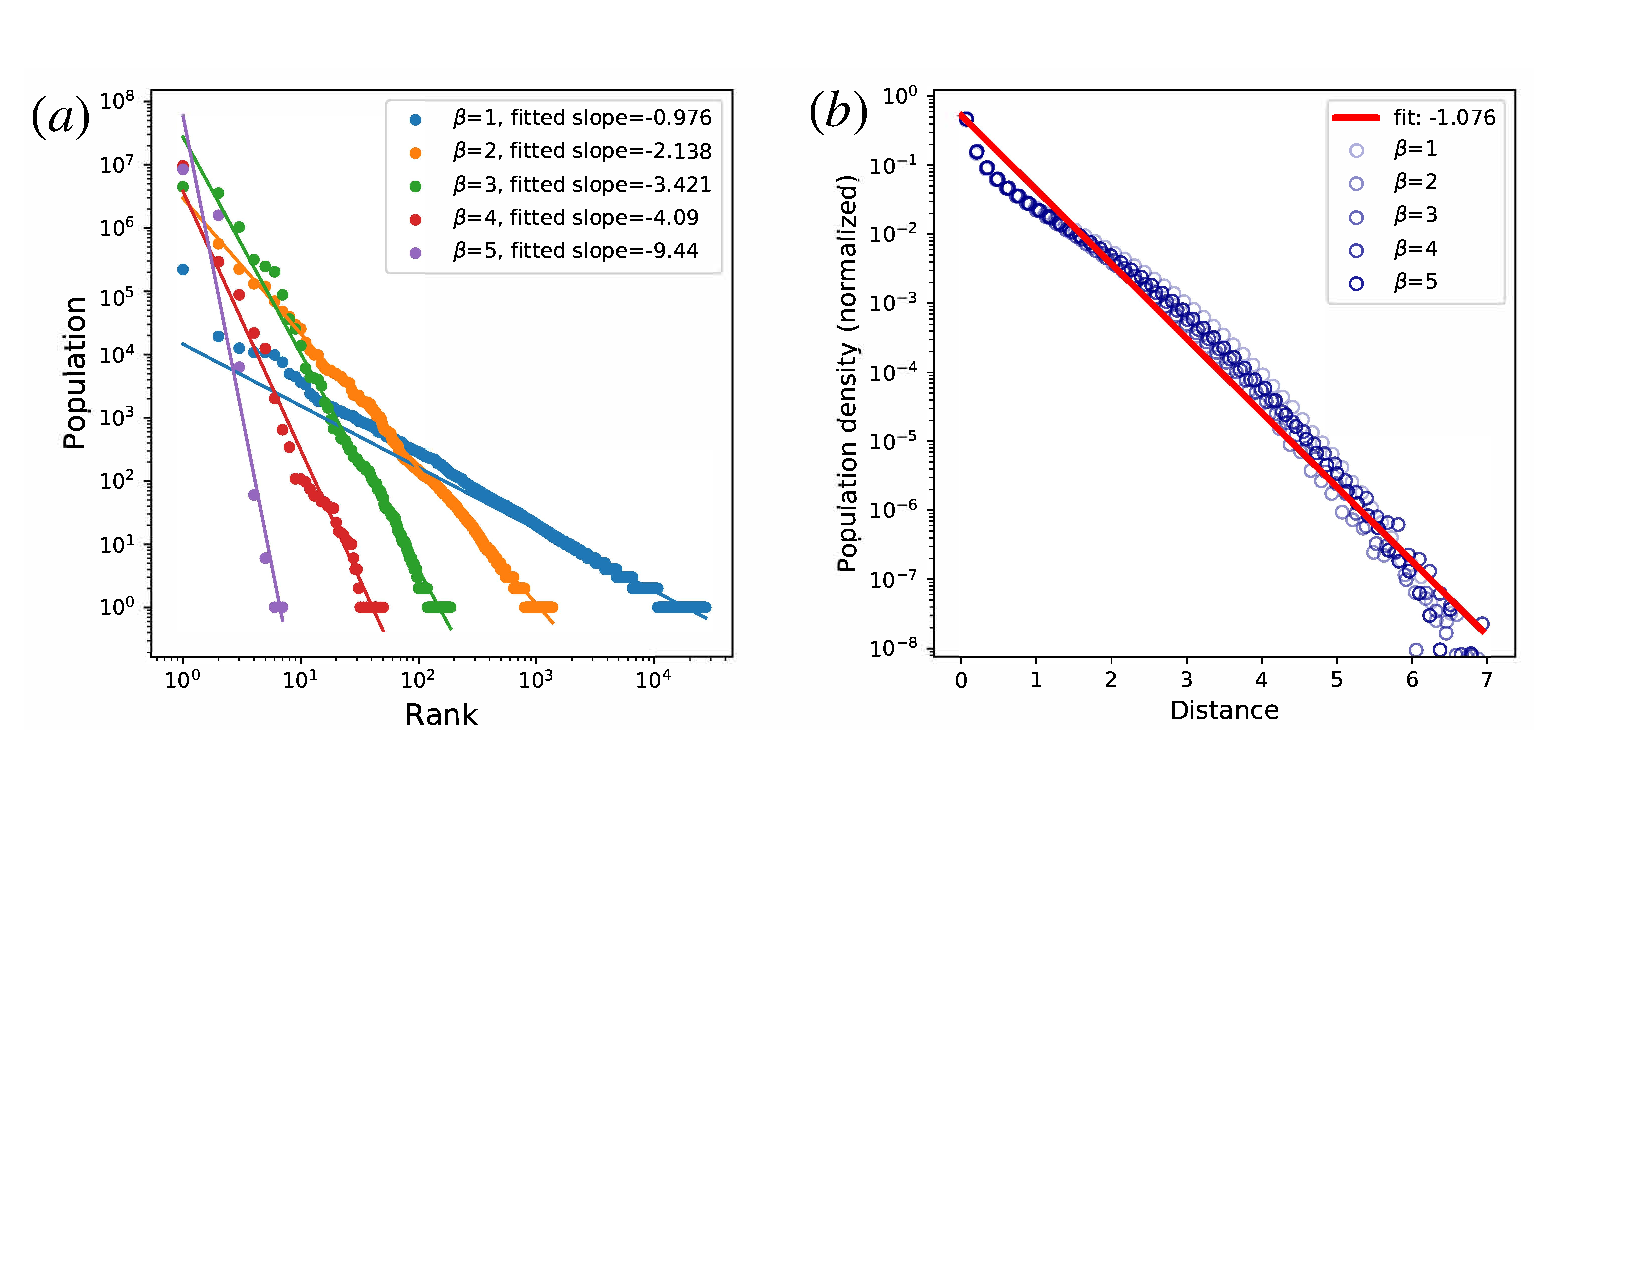
\includegraphics[width = .99\linewidth]{pics/zipf_clark.pdf}
	\caption{\textbf{(a)} The distribution of population among cities. In the simulation we take $N^* = 10^5$ and alternate $\beta$s. The realistic Zipf's coefficient is reproduced when $\beta\approx 1$. The theoretical predictions of the slopes are $-\beta$, and is well approximated when $\beta$s are small. Larger $\beta$ reduce the chance of latter city's emergence. Thus the spatial aspects of the SYM strengthen inequality. This result confirms that Zipf's law is valid for growing urban systems where all cities share the same rate to grow. From the other master equation we analyze that this observation vanishes if total growing force is finite. \textbf{(b)} The population distribution as a function of distance from a district's center. The vertical axis is logarithmic processed, which represents the exponential decaying of population distribution. Regardless of the finite-sample effect, we fit the middle part of spatial population density to the exponential distribution with a slope of $-1.076$.}
	\label{Fig2}
\end{figure}

%% Clark
% [WHAT'S THE LOGIC SENTENCE FOR THE FOLLOWING PARA? I.E., WHAT'S THE CONNECTION BETWEEN THE FOLLOWING TO ABOVE-MENTIONED THINGS?]
SYM also revisits Clark's law in urban studies~\cite{clark1951urban}. In SYM, population density evolves as two-dimensional diffusion within a city\cite{doi:10.1137/0150099}, where we can focus the density's growth on each axis from the oldest citizens of a city. Let $
(d)$ denote the active population density of locations at the distance $d$ from a city center, and $t_n$ as the time for the $n$'th citizen to generate, we have 
\begin{align}
	\rho_{t_{n+1}}(d) = (\rho_{t_{n}}(d-r) + \rho_{t_{n}}(d+r) )/2.\label{loc_den}  
\end{align} By re-scaling time as $\tau_n = t_n\cdot (k\beta_1+N\beta_2)/T$, for a sufficient large $T$, this equation results in an exponential decay of density
\begin{align}
	\rho(d)\sim e^{-\alpha d}\label{clark_eq}.
\end{align} Details are presented in \textit{SI}. 

A direct implication of Clark's law is the competition strengths at urban edges, which also influence the local Zipfian exponents. From Clark's law, the population density is just a function of city's age and the distance from urban center. Specifically, the density at the edges is important since it determines the competition advantages for space. The population within an edging cell of city $j$ is estimated by $e^{(T-T_j)}\int_{d}^{d+1}\rho(r)dr/(2\pi d)$, where $T_j$ is the emerging time of city $j$. We also have the waiting time $T_{n+1}-T_{n}\sim 1/n$, and the total population approximation $e^{\beta_1+\beta_2}$, combining which we derive the density of edging cells if time and the urban radius are given. Since the attractiveness of large urban center is larger, the edging population of large cities is actually smaller than minor cities. We validate our prediction with simulations in Fig.\@\ref{Fig2}. %[DON'T FOLLOW UP THIS PARA, WHY IT HERE, WHY IT IMPORTANT?] %We give a detailed derivation in Appendix B\ref{edge_comp}.
In supplement, larger $r$ will weaken the above prediction, since the settlement are more even, thus larger proportion of citizens live at edges. In reality, the metropolis areas over the world have very different densities. In SYM, it corresponds to the sprawl of a city with given population. It can also be taken as the area proportion for a city in the studied region. On the other hand, it also controls the spatial limit of cities given competitionless population.

\textit{The economic constraint phase}. The multi-perspective coincidence between the exponents derived in our model and those in empirical evidences of population studies indicates that only two observation scales (the generation rates of city and citizen) lead to the behaviors of regional dynamics. This means that the actual urban growth has not yet reached the constrained cases. However, preventive measures are still necessary. Thus we bring a general constraining parameter $N^*$ to further discuss the second phase of SYM, the economy constraint phase, i.e., the total population reaches $N^*$. Such setting is the abstract of many real-life rules set by global organizations such as the allowance of carbon emissions or sustainable development projects. In each city, a proportion of population are active. Here, $\sum_{i=1} N_i(t) = N^*$ for $t$ that is sufficiently large. If in some period, the minor cities generate more offspring than major ones and the superiority of remaining population within the memory kernel changes, minor city will increase its ranking, as the growing rate for each city $i$ is actually $N_i\beta_2$. As for the dynamics within memory kernel, in each city, $N_i$ acts as a random walk with absorption wall $0$, since no offspring will be expected if no nodes are left in the kernel. This result also works for single cell case within a city. Denote the population with cell $j$ of city $i$ as $m_{ij}$. According to\@\cite{durrett1999essentials}, we use a result for branching process that a cell loses its vitality if the population goes downhill under a threshold \begin{align}\rho_{threshold} = k/\beta.\end{align} This value shall be regarded as the sign for \emph{urban shrinkage}, for the edging cells have lower density according to equation\@\ref{clark_eq} thus have an exponentially higher probability to be languished. In other words, urban shrinkage shall be reasoned by limited systematic resources. 

The kernel mechanism also plays a role at the cross-city scale: The preference of larger cities is easier to fail in a system with the memory kernel. The competition for active citizens in SYM receives more than pure birth settings because the sum of active population is given as $N^*$. In other words, SYM system doesn't consider natural growth. To test this interpretation, we analyze the turnover rate, defined as the average frequency of time steps in a realization that the second largest city surpasses the largest in active population. We conduct numerical experiments, and receive power law dependence of the frequency on simulating steps, shown in Fig.\@\ref{changerate}. Moreover, the switching is more likely to happen \textit{with} a memory kernel, i.e., turnover rate decay slower in probability if the system has constraints in resource. It is also a clear result since a growing society (a society without a memory kernel) suffer less from inter-specific competition.

\begin{figure}
	\centering
	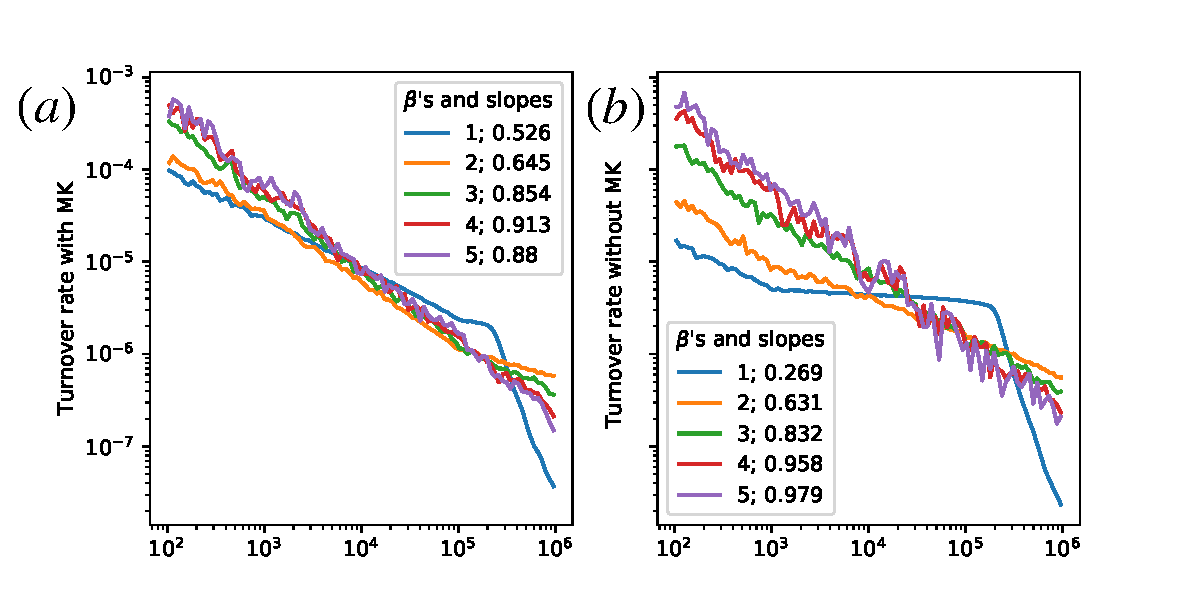
\includegraphics[width = 0.47\textwidth]{pics/in_one_now_now.pdf}
	\caption{The change rate statistics with \textbf{(a)} and without \textbf{(b)} a memory kernel. The kernel keeps turning over more often. With same $\beta$'s, a kernel-based SYM's decay in turnover rate is smaller. These results validate our prediction that with finite resource, advantages are more likely to be kept.}
	\label{changerate}
\end{figure}

The last property of SYM is the fractality of urban envelop, stately, the length of urban edges vary with the used measurement. Inspired by multi-player interaction in fractal financial market\cite{PhysRevE.65.037106}, we interpret that fractal urban boundary is driven by the competition for land at cities' edges. In SYM, the uncertain competition for space lies in parameter $r$. A larger $r$ indicates larger randomness and brings an extra advantage for minor cities, resulting in a larger fractal dimension. We apply the box counting technique to calculate the fractal dimension of urban envelops, and receive an stable output of $d_f = 1.2\pm 0.05$ with $r = 0.5$, similar to empirical results\cite{batty1992form}. We also find larger $d_f$'s for greater $r$. These results validate our hypothesis that fractal edges coexist with spatial competition. Also, this result also confirms that SYM replicates an urban system.

\textit{Discussion}. 
% 总结我们这个模型的发现有哪些,为什么我们这个好。
% Future endeavor
% 这两段是新写的。
% In this letter, we have proposed a simple model, spatial preferential growth with finite seeds, to simulate the emergence of cities and reveal the scaling laws as well as how economical dilemma would lead to spatial transitions. We account the emergence and growth of cities by adding and redistributing active population over given area. The model reveals the competition among cities in area and developmental potentials. We 
% This model leads a way in the adaptation of realistic conditions in statistical physical modeling, by regardless of the whole present population within the system, and considering only the active part of them. 
\textit{Discussion.} In summary, we have developed a spatial growth model to incorporate the effects of spatial and resource competitions in urban growth dynamics. The SYM recapitulates and generalizes earlier results from an urban growth model, including the emergence and condition of fractality, Zipf's and Clark's law. The memory kernel can shift the relative attractiveness of cities, with which the superiority of large cities stronger, while the sensitivity of the turnover rate to emergent rate $\beta$ also increases, when compared with memoryless models. The competition characterized by the memory kernel and spatial explicitation also lead to shifts in Zipfian exponent, vicissitudes, and stability criteria of large cities. These dynamics of space and resources suggests multiple avenues towards future study.

This \emph{Letter} concludes the urban system dynamics with only three key components, and presents fruitful results. The SYM leads a way in the adaptation of realistic conditions in statistical physical modeling, regardless of the whole present population within the system, and considering only the active part of them. SYM explains existing properties, such as fractality, Zipf's, and Clark's law, where we have both analytical mean-field derivations and bias analysis. More importantly, SYM predicts regional trends from a probabilistic perspective. With the simplicity of SYM, we manage to investigate the future phase transition of urban development in great detail, and explain the dilemmas of the present stage of urbanization through the competitions for systematic resource and space. The assumptions of SYM are well-held if sufficient divergence of meta-population across the world is considered. Simulations of this model can be adjust to heterogeneous geographical circumstances by applying the growing rate on each cell to the product of inherent dynamic $m_{ij}\cdot \beta_2$ and the local characteristic $c_{ij}$ to better suit for realistic conditions.

The memory kernel mechanism leads to a straightforward corollary that the reproductivity drives population's spatial transitions, as only those who are recorded in the kernel are considered as active citizens that attract new comers to his city. This result provides a bottom-up explanation for the transitions of urban centers with stochastic spatial shifts of cities' memorized people. It also tells that the economic growth is the basis of growth potentials. In reality, occasional events such as the discovery of new fossil fuel, or new technical revolutions, all lead to the growth of $N^*$. Under the circumstances of preferential attraction, if the size of the memory kernel cannot grow fast enough to match with the population, the concentration of production will go far from tolerance. 

Taking the productive aspect together in the memory kernel reveals many other properties like the age structure. The stationary age can be calculated as the average time for a new city to emerge is $(\beta_2 N^* + \beta_1 k)^{-1}$, which equals to the average losing age of the whole kernel. This result gives an instruction of the length of workable age in a given social urban system.

% 不足
Although our results are not all analytically proved, we believe it is an essential step to strip out the power of urban dynamics. The model is non-commuting, but the community structure is naturally embedded. For further consideration, we can extend the model by adding links as the volume of exploration and preferential return between cities\cite{WANG2019121921}. The model can further be extended with multi-dimensional memory kernel, allowing one citizen to be introduced if different factors\cite{tokita2020social} (i.e., the existing citizens in different dimensions of kernel) agree to allow her in the system.



\bibliography{ref.bib}

\end{document}